\documentclass[11pt,a4paper]{article}
\usepackage[margin=1in]{geometry}
\usepackage[T1]{fontenc}
\usepackage[utf8]{inputenc}
\usepackage{lmodern}
\usepackage{microtype}
\usepackage{amsmath,amssymb}
\usepackage{tikz}
\usetikzlibrary{arrows.meta,positioning}
\usepackage{booktabs,longtable,array}
\usepackage{enumitem}
\usepackage[backend=biber,style=authoryear,natbib=true,sorting=none,maxcitenames=2,maxbibnames=12,doi=true,url=false]{biblatex}
\addbibresource{references.bib}
\usepackage{xcolor}
\usepackage{hyperref}
\hypersetup{colorlinks=true,linkcolor=blue!55!black,citecolor=blue!55!black,urlcolor=blue!55!black}
\setlist[itemize]{topsep=3pt,itemsep=3pt}
\setlength{\parskip}{0.35em}
\setlength{\parindent}{1.15em}
\newcommand{\CD}{\textit{change detection}}
\newcommand{\etal}{\textit{et al.}}
\newcommand{\tabhead}[1]{\textbf{#1}}

\title{Urban Change Detection in Remote Sensing: \\Critical Literature Review and a Testable Reliability-Aware Research Proposal (2013--2026)}
\author{Research proposal and literature review draft}
\date{Literature checked: 11 November 2026}

\begin{document}
\maketitle

\begin{abstract}
Urban change detection (UCD) uses multitemporal satellite, aerial, and other geospatial observations to identify changes in buildings, infrastructure, and land use. This review and research proposal synthesize recent studies published through October 2026 and trace their methodological foundations to influential work on object-based analysis, Siamese convolutional networks, attention, and public benchmarking. The literature shows a progression from spectral and object-based comparison to deep binary segmentation, Transformer-based temporal reasoning, state-space models, and vision foundation models. The central argument is that improved feature representation alone does not guarantee operationally reliable maps of city growth: co-registration, spatial resolution, shadow and seasonal invariance, label quality, cross-city transfer, and sensitivity to vertical construction remain decisive. Building on the reviewed evidence, we propose GReST-CD: a testable model design combining change-preserving alignment, nuisance-counterfactual consistency, building-state reasoning, optional reliability-gated elevation, and calibrated selective prediction. We specify training objectives, geographic holdout experiments, ablations, failure tests, and a results-reporting template. No new experimental performance results are claimed.
\end{abstract}

\noindent\textbf{Keywords:} urban change detection; building change detection; remote sensing; bi-temporal imagery; geographic transfer; reliable change detection; optical--DSM fusion; uncertainty calibration; research methodology.

\section{Introduction and scope}

Rapid urban expansion, demolition, reconstruction, and infrastructure development require maps that can be updated more frequently than conventional cadastral surveys. Urban remote sensing addresses this need through comparisons of observations acquired at different times. Applications range from mapping new building footprints and the conversion of agricultural land to built-up surfaces to monitoring informal development and post-disaster damage. Unlike broad land-cover change detection, urban change detection must preserve building edges and separate real structural transitions from shadows, roof-reflectance differences, vegetation phenology, sensor geometry, and imperfect registration \citep{Gomroki2026,ChengReview2024}.

Let two co-registered images of a geographic region be denoted by $I_{t_1},I_{t_2}\in\mathbb{R}^{H\times W\times C}$. Binary change detection estimates a mask
\begin{equation}
  \hat{M}=f_{\theta}(I_{t_1},I_{t_2}),\qquad \hat{M}(x,y)\in[0,1],
  \label{eq:cd}
\end{equation}
where a threshold converts the probability of relevant change into a binary label. Urban semantic change detection instead estimates a class transition, such as \emph{vegetation $\rightarrow$ built-up} or \emph{building $\rightarrow$ bare land}. Building-level detection may additionally require object instances, footprints, and construction-versus-demolition direction. Two-dimensional imagery primarily reveals planimetric change, whereas digital surface models (DSMs), photogrammetric point clouds, or LiDAR can reveal height and volume change \citep{Gomroki2026}.

\paragraph{Selection principle.} This is a \emph{critical narrative review}, not a PRISMA systematic review or a complete citation-ranked bibliometric census. Recent contributions were prioritized when explicitly relevant to urban or building change detection, and older studies were selected because they introduced widely used methods or benchmarks. The discussion is ordered from \emph{newest to foundational}, broadly consistent with a request to work backward from recent work toward frequently referenced classics. \textbf{The sequence is not an audited ranking by citation count}; citation totals vary among Google Scholar, Scopus, OpenAlex, and other indexes and with the retrieval date.

\section{Recent advances, reviewed from newest to older work}

\subsection{2026: urban-specific spectral learning, foundation features, and measurement discipline}

Among recent urban-specific studies, \citet{Pal2026} proposed a multispectral Siamese U-Net for urban change mapping with Sentinel-2 RGB and near-infrared (NIR) observations, dynamic spatial cropping, and a combined binary-cross-entropy--Dice loss. On its evaluated imagery, it reported a precision of 88.65\% and argued that NIR helps distinguish anthropogenic modification from vegetation-related spectral changes. Its contribution is practical: in large-area municipal monitoring, inexpensive, repeatable multispectral coverage and class-imbalance-aware training may matter more than adding model complexity. A fundamental limitation is spatial scale: Sentinel-2's 10-m bands are appropriate for neighborhood-scale expansion and larger structures but cannot generally resolve individual small-building boundaries as reliably as sub-meter imagery.

In a September 2026 study on LEVIR-CD, \citet{Tiwari2026} combined a Siamese ResNet50 encoder, temporal-spatial attention, an SNUNet-style decoder, and channel attention. Critically, its controlled ablation showed that preserving native spatial detail through tiling rather than resizing increased its $F_1$ by 17.11 percentage points (73.24\% to 90.35\%). The final model achieved 90.35\% $F_1$ on its stated official test protocol, closely matching a simpler ResNet50 U-Net baseline (90.38\%). This is an important corrective to architecture-centered narratives: preprocessing and transparent baseline comparison can dominate marginal architectural gains. These values are \emph{study-specific} and must not be treated as a uniform leaderboard across papers.

\citet{ChengHsu2026} introduced \emph{ChangeDINO}, adapting DINOv3-derived representations to multiscale Siamese building change detection. The study illustrates the growing use of large pretrained visual encoders when changed-pixel labels are scarce. Similarly, \citet{Zhu2026} proposed \emph{ChangeViT}, using pretrained plain vision Transformers with mechanisms to recover fine-scale details; tests include the urban-building benchmarks LEVIR-CD and WHU-CD. These approaches suggest that pretrained representations can improve scene understanding, although robust transfer to different cities, viewing conditions, and sensor resolutions cannot be assumed from in-domain benchmark scores alone.

At the review level, \citet{Gomroki2026} compared 2D and 3D urban change detection. Its key distinction is particularly relevant to dense vertical cities: a footprint may remain nearly constant while an additional floor or rooftop structure changes building volume. Thus, binary 2D building-change masks and 3D structural-change measurements are complementary rather than interchangeable.

\subsection{2025: semantic meaning, geometry, synthetic labels, and efficient sequence models}

\citet{Jiang2025} proposed \emph{AdaptVFMs-RSCD}, combining Segment Anything Model (SAM) and CLIP representations to move beyond binary change masks toward semantic information. This addresses a fundamental municipal question: rather than simply determining \emph{where} something changed, planners need to know \emph{what} changed. Yet vision--language models inherit limitations related to geospatial domain mismatch and prompt or vocabulary choice; therefore, label definitions and independent verification remain important.

Geometric knowledge is another emerging direction. \citet{Quan2025} incorporated relative depth information produced with a foundation-model-based approach into change detection. In more explicitly urban settings, \citet{Fu2025} fused DSM-derived geometry, optical imagery, and vegetation information in \emph{DDDMNet} to better distinguish building changes from spectral artifacts. These studies point to the usefulness of elevation-sensitive features where shadowing, roof replacement, and vertical construction confuse purely optical methods. The trade-off is that DSMs or depth estimates may be noisy, spatially inconsistent, or unavailable for both dates.

\citet{WangWu2025} introduced \emph{BiUnet-Dense} for urban change detection, combining deep feature extraction, dense connections, and temporal modeling. This represents a continuing effort to make CNN-based methods more robust to changing spatial appearance without depending solely on global attention. Separately, \citet{Paranjape2025} presented an efficient Mamba-based Siamese change detector, reflecting interest in long-range spatial interactions without the full quadratic attention cost of conventional Transformers.

A different response to scarce labeled data was proposed by \citet{Benidir2025}. Their \emph{HySCDG} pipeline and \emph{FSC-180k} hybrid dataset use real very-high-resolution images together with semantically guided synthetic modifications for semantic change detection. Such augmentation is promising for uncommon urban transition types, but synthetic realism and transfer to independently sampled cities must be evaluated carefully; artificial changes may not reproduce the optical and geometric signatures of actual construction activity.

\subsection{2024: state-space models and vision-language / zero-shot change detection}

The 2024 literature marked a shift beyond CNN--Transformer hybrids. \citet{ChenMamba2024} developed \emph{ChangeMamba}, a state-space-model family including MambaBCD (binary), MambaSCD (semantic), and MambaBDA (building damage assessment). Its main contribution is spatiotemporal context modeling that can remain computationally attractive for larger imagery. However, a favorable theoretical complexity argument does not by itself establish lower end-to-end operational cost once tiling, preprocessing, and memory are included.

For multimodal reasoning, \citet{Dong2024} proposed \emph{ChangeCLIP}, using vision--language representation learning to bring text-associated semantic information into remote sensing change detection. In parallel, \citet{Zheng2024} introduced \emph{AnyChange}, a training-free adaptation of SAM using bi-temporal latent matching to support zero-shot change detection. Both directions reduce reliance on conventional exhaustively labeled training sets, but their ability to correctly identify subtle construction, temporary objects, or sensor-induced pseudo-changes requires context-specific validation. The broad methodological landscape, including supervision modes, multimodal inputs, and evaluation limitations, was summarized by \citet{ChengReview2024}.

\subsection{2021--2022: the Transformer and modern benchmark consolidation}

A series of influential works established the baselines against which recent innovations are frequently measured. \citet{ChenBIT2022} introduced the \emph{Bitemporal Image Transformer} (BIT), compressing learned scene features into a smaller set of semantic tokens, modeling temporal relationships by Transformer, then projecting contextual information back to pixels. This addressed the restricted spatial context of local convolutional encoders. \citet{Bandara2022} developed \emph{ChangeFormer}, a hierarchical Transformer-based Siamese encoder with a multilayer-perceptron decoder and multiscale feature fusion. The latter has been widely used as a strong contextual baseline in building change detection.

At the same time, \citet{Fang2022} proposed \emph{SNUNet-CD}, a densely connected Siamese architecture designed to preserve multilevel spatial details for very-high-resolution changes. Importantly, the continued adoption of SNUNet-style components in later work \citep{Tiwari2026} shows that convolutional architectures have not simply been replaced by foundation models. For medium-resolution urban monitoring, \citet{Basavaraju2022} proposed \emph{UCDNet} on bi-temporal multispectral Sentinel-2 imagery, emphasizing the usefulness of spectral information and accessible data for built-up land monitoring.

Dataset design became equally consequential. \citet{Shen2021} introduced \emph{S2Looking}, with 5,000 bi-temporal side-looking satellite image pairs and more than 65,000 annotated change instances, deliberately challenging methods trained on near-nadir imagery. Although much of S2Looking contains rural scenes rather than dense cities, its off-nadir geometry exposes a major operational problem for tall urban buildings: viewpoint-induced apparent displacement can mimic structural change.

\subsection{2018--2020 and earlier: influential foundations}

\citet{ChenShi2020} introduced \emph{STANet}, which learns spatial--temporal pixel relationships through attention, and the \emph{LEVIR-CD} benchmark. LEVIR-CD contains 637 co-registered 1,024$\times$1,024 image pairs from several Texas urban regions at approximately 0.5-m ground sample distance, with annotations emphasizing building additions and removals. It helped turn urban building change detection into a reproducible deep-learning benchmark. Nevertheless, success on a limited set of related metropolitan regions does not automatically demonstrate performance under different architecture, construction materials, climates, or imaging geometries.

\citet{Ji2019} published the Wuhan University (WHU) building imagery resource and associated fully convolutional building-extraction work; its building change detection subset became another widely used testbed. The paper helped normalize access to annotated high-resolution aerial change observations. \citet{Daudt2018} established important early-fusion and Siamese fully convolutional baselines. Their paired-encoder design remains central to current networks, because it enables before/after representations to be compared with shared feature extractors. Before end-to-end learning became dominant, \citet{Hussain2013} synthesized pixel-based and object-based techniques, explaining why spectral differencing often requires object context to generate meaningful maps. These studies are historically and methodologically influential, but the current review does \emph{not} claim they form a verified numerical ``most-cited'' ranking.

\section{Comparative synthesis of representative studies}

\renewcommand{\arraystretch}{1.13}
\small
\begin{longtable}{@{}>{\raggedright\arraybackslash}p{0.11\textwidth}>{\raggedright\arraybackslash}p{0.23\textwidth}>{\raggedright\arraybackslash}p{0.31\textwidth}>{\raggedright\arraybackslash}p{0.265\textwidth}@{}}
\caption{Selected urban-relevant studies in reverse chronological order. Limitations are the review's synthesis, not necessarily direct statements by the original authors.}\label{tab:studies}\\
\toprule
\tabhead{Year} & \tabhead{Study / family} & \tabhead{Main contribution to urban change detection} & \tabhead{Primary limitation or open question} \\
\midrule
\endfirsthead
\multicolumn{4}{l}{\small\emph{Table \thetable\ continued}}\\
\toprule
\tabhead{Year} & \tabhead{Study / family} & \tabhead{Main contribution} & \tabhead{Limitation / question} \\
\midrule
\endhead
\bottomrule
\endfoot
2026 & \citet{Pal2026}; multispectral Siamese U-Net & NIR and dynamic crops for Sentinel-2 urban change; class-imbalance-aware loss & Moderate spatial resolution limits small-building mapping \\
2026 & \citet{Tiwari2026}; SNUNet/attention & Strong tiling ablation; transparent comparison with a simpler baseline & Results remain benchmark-specific; model complexity needs justification \\
2026 & \citet{ChengHsu2026}; ChangeDINO & DINOv3-derived representations for building changes & Cross-city and cross-sensor adaptation need study \\
2026 & \citet{Zhu2026}; ChangeViT & Pretrained ViTs with multiscale detail recovery & Inference cost and domain robustness \\
2025 & \citet{Jiang2025}; SAM + CLIP & From binary change to semantic descriptions & Domain mismatch and ambiguous semantic labels \\
2025 & \citet{Quan2025}; depth-assisted CD & Geometry-aware discrimination & Estimated depth quality and temporal consistency \\
2025 & \citet{Fu2025}; DDDMNet & Optical--DSM--vegetation fusion for urban buildings & Availability and alignment of repeated height data \\
2025 & \citet{Benidir2025}; HySCDG & Hybrid real/synthetic semantic labels & Sim-to-real domain gap \\
2025 & \citet{Paranjape2025}; Mamba Siamese & Efficient long-range feature interactions & End-to-end resource use and external validation \\
2024 & \citet{ChenMamba2024}; ChangeMamba & State-space binary, semantic, and damage tasks & Consistent protocols across tasks and modalities \\
2024 & \citet{Dong2024}; ChangeCLIP & Vision--language semantics for change features & Prompt dependence and geographic shift \\
2024 & \citet{Zheng2024}; AnyChange & SAM-based training-free / zero-shot comparison & Fine-grained urban edits and false change \\
2022 & \citet{ChenBIT2022}; BIT & Efficient semantic-token temporal Transformer & Resolution-dependent fine-edge recovery \\
2022 & \citet{Bandara2022}; ChangeFormer & Hierarchical Transformer Siamese framework & Compute needs and dataset-specific tuning \\
2022 & \citet{Fang2022}; SNUNet-CD & Dense multiscale Siamese feature fusion & Limited semantic characterization of change \\
2022 & \citet{Basavaraju2022}; UCDNet & Multispectral Sentinel-2 urban change & Medium-resolution footprint ambiguity \\
2020 & \citet{ChenShi2020}; STANet / LEVIR-CD & Spatial--temporal attention and benchmark & Narrow scene and geography distribution \\
2019 & \citet{Ji2019}; WHU dataset & High-resolution building extraction/change resource & Aerial-to-satellite transfer not guaranteed \\
2018 & \citet{Daudt2018}; FC Siamese & End-to-end paired CNN baselines & Local context and spectral pseudo-change \\
2013 & \citet{Hussain2013}; classic review & Pixel--object taxonomy and methodological framing & Predates deep representation learning \\
\end{longtable}
\normalsize

\section{Datasets, evaluation, and comparability}

\begin{table}[htbp]
\centering
\small
\caption{Common benchmark families and their relevance for city monitoring.}
\label{tab:data}
\begin{tabular}{@{}>{\raggedright\arraybackslash}p{0.17\textwidth}>{\raggedright\arraybackslash}p{0.31\textwidth}>{\raggedright\arraybackslash}p{0.40\textwidth}@{}}
\toprule
\tabhead{Dataset} & \tabhead{Strength} & \tabhead{Caution for urban deployment} \\
\midrule
LEVIR-CD \citep{ChenShi2020} & High-resolution, annotated building additions/removals; many reproducible comparisons & Limited Texas-region distribution; tiles from nearby places can be correlated \\
WHU-CD \citep{Ji2019} & Very-high-resolution aerial building change; fine spatial detail & Same-sensor aerial conditions may not transfer to oblique satellite imaging \\
S2Looking \citep{Shen2021} & Off-nadir imaging, varied view and illumination & Many rural scenes; not a substitute for city-specific validation \\
OSCD \citep{Basavaraju2022} & Multispectral Sentinel-2, diverse urban environments & Coarser pixel size; annotations and task definitions vary by study \\
FSC-180k \citep{Benidir2025} & Real plus generated semantic change data for pretraining & Synthetic shifts must be tested against real future observations \\
\bottomrule
\end{tabular}
\end{table}

For binary maps, changed-class precision, recall, $F_1$, and intersection over union (IoU) are more informative than overall accuracy when most urban pixels are unchanged:
\begin{equation}
 P=\frac{TP}{TP+FP},\quad R=\frac{TP}{TP+FN},\quad
 F_1=\frac{2PR}{P+R},\quad
 \mathrm{IoU}=\frac{TP}{TP+FP+FN}.
 \label{eq:metrics}
\end{equation}
Object-level precision/recall, building polygon quality, semantic transition consistency, and map uncertainty are also needed when outputs will feed a geographic information system (GIS). Scores from different studies should \emph{not} be ranked unless they share identical image/label versions, geographic splits, input bands, spatial resolution, threshold selection, and evaluation code. In particular, patch-wise random splits can leak spatial context from nearby regions into training and testing. Report both processing resolution and effective ground sample distance, and never interpret a result for a 0.5-m urban footprint dataset as directly interchangeable with one for 10-m Sentinel-2 urban expansion.

\section{Critical research gaps}

\paragraph{Geographic and temporal generalization.} Benchmarks tend to reuse a few imagery sources and development patterns; cities vary in roofing materials, building density, topography, and seasons. Training/validation/testing by \emph{held-out city and acquisition period}, rather than random patches, provides a more realistic estimate of operational transfer. Cross-sensor studies are especially needed when historic imagery comes from aerial or commercial sensors and recent observations from Sentinel-2 or alternative providers.

\paragraph{False changes versus true structural changes.} Parallax from off-nadir imagery, shadow movement, seasonal vegetation, road resurfacing, and nonuniform registration can all look like building change. S2Looking and recent geometry-based methods motivate explicit geometric alignment, shadow-awareness, and confidence calibration \citep{Shen2021,Quan2025}. Performance on difficult subsets should be reported separately instead of hiding failure cases inside an aggregate $F_1$.

\paragraph{Missing height and city function.} Two-dimensional maps reveal changed roofs and footprints but often miss renovation, vertical densification, or replacement of a low-rise with a taller structure on the same footprint. Joint optical--DSM or optical--LiDAR models are a promising solution, but evaluation data must preserve comparable vertical reference systems and acquisition quality \citep{Gomroki2026,Fu2025}.

\paragraph{Semantic and low-label learning.} Binary labels cannot distinguish new housing from industrial development or a demolition from vegetation clearance. VLM-based change detection and hybrid data generation may help \citep{Jiang2025,Benidir2025}, but city-specific ontologies, cross-city calibration, and reliable descriptions of change are still necessary. Zero-shot systems should be tested on unseen urban categories rather than only unseen imagery from familiar benchmarks.

\paragraph{Efficiency, trust, and reproducibility.} Larger networks are not automatically better for repeat continental-scale mapping. The 2026 ablation of \citet{Tiwari2026} is a reminder to control for input tiling, clipping, threshold selection, and training instability. Evaluations should also report total runtime (not only neural-network latency), GPU memory, parameter counts, missing-data handling, uncertainty, and human verification needs.

\section{Recommended research direction for a city-scale study}

A defensible study could compare \emph{three tiers} of models on precisely matched imagery: (i) a fully convolutional Siamese baseline \citep{Daudt2018}, (ii) a contextual attention/Transformer baseline \citep{ChenShi2020,ChenBIT2022,Bandara2022}, and (iii) a state-space or pretrained foundation-model alternative \citep{ChenMamba2024,ChengHsu2026}. For each tier, use a common preprocessing and loss/evaluation pipeline. Evaluate separately on (a) dense inner-city redevelopment, (b) suburban infill, (c) peripheral urban expansion, and (d) cities completely absent from the training data.

The experimental unit should be a \emph{geographically separated scene or city}, not an arbitrary crop. At minimum, report changed-class $F_1$/IoU, building-object recall, false alarms from shadows and vegetation, spatial registration error, and inference cost. If height data exist, extend the labels to footprint change versus height-only change. This design would directly test whether newly introduced context models improve \emph{transferable} urban understanding, not merely optimization on a heavily reused public benchmark.

\section{Proposed research: GReST-CD for reliable urban structural transitions}
\label{sec:proposed}

\subsection{Research question and contribution hypothesis}

\textbf{Research question.} Can a model that explicitly separates residual geometric error, appearance-only perturbations, physical building change, and input-data reliability generalize better to unseen cities than a conventional single-head change detector, without sacrificing boundary fidelity or deployability?

We propose \emph{GReST-CD} (\textbf{G}eometry- and \textbf{Re}liability-aware \textbf{S}tructural \textbf{T}ransition Change Detection), a \emph{research hypothesis and implementable model design}, not an experimentally validated architecture. The core idea is to make a prediction depend on evidence of a \emph{physical transition}, rather than on unconstrained spectral differences, and to return an explicit ``review required'' decision for unreliable regions. GReST-CD combines: (1) change-preserving residual alignment; (2) nuisance-counterfactual learning that leaves true urban edits unchanged; (3) date-specific footprint reasoning for construction and demolition \emph{when corresponding supervision exists}; (4) reliability-gated, optional normalized-height evidence; and (5) calibrated selective mapping with a transparent coverage--error trade-off.

\paragraph{Relationship to recent studies and limits of originality.} Joint alignment and change learning have already been studied by \citet{Lu2026}; uncertainty-guided building change detection by \citet{LiUncertainty2025}; edge-aware modeling by \citet{Holail2025}; optical--DSM fusion by \citet{Fu2025}; and cross-city semi-supervision and evaluation by \citet{Srivastava2026}. Consequently, \emph{none} of these ingredients alone is claimed as new. The \emph{proposed contribution to test} is their integration under explicit causal-like nuisance interventions, optional-height gating, structurally consistent direction labels, and an operational abstention protocol, all evaluated together under geographic holdouts. Novelty and performance superiority would require a broader prior-art audit and actual controlled experiments.

\subsection{Task definition and observability}

Let $I_1,I_2\in\mathbb{R}^{H\times W\times C}$ be two radiometrically normalized, approximately co-registered optical images; $V_1,V_2\in\{0,1\}^{H\times W}$ denote usable-pixel masks (clouds, no-data, and extreme occlusion are invalid). Optional normalized digital surface models $H_1,H_2$ have independent validity/quality layers $V_H$ and $Q_H\in[0,1]^{H\times W}$. All maps are projected to a documented common coordinate system and ground sample distance. Target outputs are: a binary footprint-change probability $p_{\rm fp}$; when supervised, \emph{new}, \emph{removed}, and \emph{unchanged} building status; an optional height-only-change probability $p_{\rm ht}$; and an uncertainty/review flag. A changed road or vegetation patch is \emph{not} a positive building-footprint example unless the chosen label ontology explicitly includes it.

\textbf{Identifiability condition.} A single building-change mask alone does \emph{not} label which date contains the building: a direction-aware head needs separate dated building masks or independently verified construction/demolition instances. Height-only modifications cannot be validated using LEVIR-CD or WHU-CD's usual 2D binary-change masks; they require two comparable elevation measurements and a height-change annotation protocol. When either kind of supervision is missing, its task-specific loss and corresponding claims are disabled, not imputed.

\subsection{Architecture and data flow}

\begin{figure}[htbp]
\centering
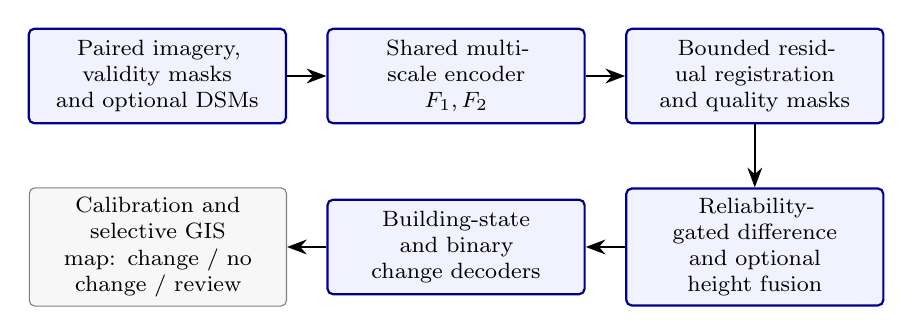
\begin{tikzpicture}[
  node distance=5mm and 5mm,
  stage/.style={draw=blue!55!black,fill=blue!5,rounded corners=2pt,thick,align=center,font=\footnotesize,text width=0.25\textwidth,minimum height=12mm},
  smallstage/.style={draw=black!50,fill=black!3,rounded corners=2pt,align=center,font=\footnotesize,text width=0.25\textwidth,minimum height=12mm},
  arr/.style={-{Stealth[length=2.5mm]},thick}
]
\node[stage] (a) {Paired imagery, validity masks\\and optional DSMs};
\node[stage,right=of a] (b) {Shared multiscale encoder\\$F_1,F_2$};
\node[stage,right=of b] (c) {Bounded residual registration\\and quality masks};
\node[stage,below=8mm of c] (d) {Reliability-gated difference\\and optional height fusion};
\node[stage,left=of d] (e) {Building-state and binary\\change decoders};
\node[smallstage,left=of e] (f) {Calibration and selective GIS\\map: change / no change / review};
\draw[arr] (a)--(b);\draw[arr] (b)--(c);
\draw[arr] (c)--(d);\draw[arr] (d)--(e);\draw[arr] (e)--(f);
\end{tikzpicture}
\caption{Conceptual GReST-CD pipeline. Height evidence is optional and is fused only when valid. The figure is an architecture proposal, not a trained-system result.}
\label{fig:grest}
\end{figure}

\paragraph{Stage A: change-preserving alignment.} A shared encoder $E_{\theta}$, initialized from a standard Siamese CNN or a frozen/pretrained visual backbone, produces multiscale features $F_t^s=E_{\theta}^s(I_t)$. A lightweight registration head predicts a bounded residual displacement field $d^s(x)$; the second feature map is resampled as
\begin{equation}
 \bar F_2^s(x)={\cal W}(F_2^s,d^s)(x),\qquad
 d^s=\operatorname{clip}(A_{\phi}(F_1^s,F_2^s),-d_{\max},d_{\max}).
 \label{eq:align}
\end{equation}
The \emph{coarse} image alignment occurs before learning. The residual head is only allowed to correct small acquisition offsets: $d_{\max}$ is set from the observed residual registration tolerance, rather than tuned on the test set. This prevents a flexible warp from moving or erasing newly constructed buildings to minimize feature differences. Define $q_{\rm uc}=\operatorname{stopgrad}[(1-\tilde p_{\rm fp})\,q_{\rm reg}\,V_1V_2]$, where $\tilde p_{\rm fp}$ is a detached preliminary change estimate and $q_{\rm reg}$ indicates reliable, nonoccluded correspondence. In supervised training, ground-truth unchanged regions can supervise or warm-start this mask. The alignment loss becomes
\begin{equation}
 {\cal L}_{\rm reg}=\frac{\sum_x q_{\rm uc}(x)\,\rho(F_1(x)-\bar F_2(x))}{\epsilon+\sum_x q_{\rm uc}(x)}
 +\lambda_{\rm sm}\sum_x\|\nabla d(x)\|_1,
 \label{eq:regloss}
\end{equation}
with a robust Huber/Charbonnier penalty $\rho$ and a spatial-smoothness term. To avoid self-fulfilling zero-confidence masks, correspondence quality is derived from independent matching diagnostics and known synthetic geometric corruptions, with gradients stopped through $q_{\rm uc}$. Models should be tested for \emph{over-alignment} on genuine construction events.

\paragraph{Stage B: quality-gated structural evidence.} Let $D_o$ contain $|F_1-\bar F_2|$, $F_1\odot\bar F_2$, and multiscale context. A learned reliability indicator $q_o(x)\in[0,1]$, trained against known nuisance/validity perturbations rather than only binary change labels, modulates optical evidence. If a comparable height pair exists, define $\Delta H={\cal W}(H_2,d_H)-H_1$ in a common vertical datum and
\begin{equation}
 D(x)=\big[q_o(x)D_o(x),\;V_H(x)Q_H(x)\,\psi(\Delta H(x)),\;V_H(x)Q_H(x)\big].
 \label{eq:fusion}
\end{equation}
Here $\psi$ encodes signed height differences, and $Q_H$ is a quality estimate from DSM metadata, stable-surface residuals, and predicted measurement uncertainty; \emph{it is not decreased merely because a large true height change is observed}. Missing height input is represented by a zero evidence tensor \emph{plus a missingness bit}, not a fictitious zero height change. Dropout of the height modality during training teaches the optical path to remain functional.

\paragraph{Stage C: date-specific transitions and map outputs.} A shared decoder predicts per-date building probabilities $b_1,b_2$ if date-specific supervision exists. Assuming conditionally independent Bernoulli decisions \emph{for the purpose of deriving an auxiliary output}, construction and demolition probabilities are
\begin{equation}
 p_{\rm new}=(1-b_1)b_2,\qquad
 p_{\rm rem}=b_1(1-b_2),\qquad
 p_{\rm xor}=p_{\rm new}+p_{\rm rem}.
 \label{eq:transition}
\end{equation}
A primary binary footprint head $p_{\rm fp}$ remains available on binary-only datasets. The consistency penalty $\|p_{\rm fp}-p_{\rm xor}\|_1$ is activated \emph{only} for datasets with per-date building supervision; otherwise an arbitrary construction/demolition split would be nonidentifiable. If height labels exist, an additional head detects height-only structural changes on regions with stable footprints, and outputs are reported separately rather than silently folded into a 2D footprint benchmark.

\paragraph{Stage D: counterfactual nuisance consistency and selective reporting.} Generate two versions of the \emph{same} labeled image pair by perturbing acquisition properties---illumination, color response, physically plausible shadows, mild sensor noise, and known subpixel shifts---without editing actual building footprints. With $T^{-1}$ mapping augmented outputs back to original coordinates, encourage
\begin{equation}
 {\cal L}_{\rm inv}=\frac{\sum_{x\in\Omega_v}w(x)\,
  \operatorname{JS}\big(p_{\rm fp}(I_1,I_2)(x),
    T^{-1}p_{\rm fp}(T_1I_1,T_2I_2)(x)\big)}
 {\epsilon+\sum_{x\in\Omega_v}w(x)},
 \label{eq:invariance}
\end{equation}
where JS denotes Jensen--Shannon divergence between two Bernoulli predictive distributions, and $w$ excludes newly occluded/no-data pixels. Independently augmenting the dates is important: applying the same color change to both cannot teach invariance to differing sun or sensor conditions. Do not use synthetic building edits as nuisance transformations. At inference, calibrate the change-head probabilities by temperature scaling on \emph{training-domain validation/calibration regions}. Use a small deep ensemble or Monte Carlo dropout to estimate predictive disagreement $u(x)$; report a map label only when $u(x)\leq\tau_u$ and the data-validity criteria hold. Otherwise, emit \emph{review required}. This is selective prediction, \emph{not} a guaranteed conformal error bound on unseen cities.

\subsection{Training and optimization}

For valid pixels $\Omega_v$, combine class-balanced binary cross-entropy and soft Dice loss for footprint change:
\begin{equation}
 {\cal L}_{\rm fp}=\lambda_{\rm bce}\,{\rm BCE}_w(p_{\rm fp},Y_{\rm fp})
  +\lambda_{\rm dice}\big(1-\operatorname{Dice}(p_{\rm fp},Y_{\rm fp})\big).
 \label{eq:footloss}
\end{equation}
On datasets with compatible supervision, add per-date segmentation loss $\mathcal L_{\rm date}$, consistency $\mathcal L_{\rm trans}$, and height loss $\mathcal L_{\rm ht}$; otherwise their supervision masks are zero. The complete masked objective is
\begin{equation}
 \mathcal L=\mathcal L_{\rm fp}+\alpha\mathcal L_{\rm reg}
 +\beta\mathcal L_{\rm inv}+m_{\rm date}(\gamma\mathcal L_{\rm date}+\delta\mathcal L_{\rm trans})
 +m_{\rm ht}\zeta\mathcal L_{\rm ht}+\eta\mathcal L_{\rm quality},
 \label{eq:total}
\end{equation}
where $m_{\rm date},m_{\rm ht}\in\{0,1\}$ denote actual annotation/modality availability, not learned proxies. $\mathcal L_{\rm quality}$ uses ground-truth synthetic corruption masks and registered control points where available, so reliability gating is not optimized to suppress all difficult pixels. We propose (i) a 10-epoch warm-up of the baseline footprint model with coarse registration frozen, (ii) joint feature/alignment optimization, and (iii) nuisance consistency and uncertainty calibration. All loss weights must be chosen on validation regions and ablated; their numerical values are \emph{hyperparameters to be determined}, not claimed optima.

\section{Experimental methodology and reproducibility plan}
\label{sec:experiment}

\subsection{Datasets, splits, and annotation design}

\begin{table}[htbp]
\centering\footnotesize
\caption{Planned evaluation settings. ``Available'' refers to the required type of data, not to data already downloaded or experiments completed.}
\label{tab:protocol}
\begin{tabular}{@{}>{\raggedright\arraybackslash}p{0.21\textwidth}>{\raggedright\arraybackslash}p{0.31\textwidth}>{\raggedright\arraybackslash}p{0.36\textwidth}@{}}
\toprule
\tabhead{Setting} & \tabhead{Main purpose} & \tabhead{Important restriction}\\
\midrule
LEVIR-CD / WHU-CD & Comparable optical footprint-change baselines & Binary change only under standard labels; no validated direction or height-only score \\
S2Looking & Stress test for off-nadir geometry and shadow artifacts & Not exclusively urban; use area-stratified reporting \\
ICCD (if accessible) \citep{Srivastava2026} & Geographic transfer across Indian cities & Confirm licensing, access, labels and city-level partitions before use \\
Multi-city held-out study & Realistic transfer and development-pattern diversity & Acquire independent permissions and \emph{new} city/site labels \\
Matched optical + two-date DSM subset & Test change in height without footprint growth & Require same horizontal/vertical datum and independent elevation truth \\
\bottomrule
\end{tabular}
\end{table}

Public data should retain their official train/validation/test splits when making published-benchmark comparisons, with \emph{no} tile leakage. Geographic-generalization experiments require a separate city-diverse dataset or suitable city-labeled partitions; LEVIR-CD alone does not establish leave-one-city-out transfer. For a newly collected city corpus, reserve entire cities for testing, choose hyperparameters using distinct validation cities, and enforce a spatial buffer between sites. Record all sensors, acquisition dates, ground sample distance, cloud/occlusion masks, datum transforms, geographic bounds, and verification status. For change direction, independently digitize building footprints at each date and reconcile disagreements with a second annotator. For height-only change, use comparable DSMs or field-verified elevation, estimate vertical error from stable surfaces, and predefine a change threshold above sensor noise.

\subsection{Baselines, training settings, and controlled stress tests}

Compare with a well-tuned Siamese FCN \citep{Daudt2018}, STANet \citep{ChenShi2020}, BIT \citep{ChenBIT2022}, ChangeFormer \citep{Bandara2022}, and a current pretrained encoder such as ChangeDINO \citep{ChengHsu2026}. Compare against \citet{Lu2026} where implementation and identical input conditions are accessible. For a height-equipped cohort, include a DSM-based method such as DDDMNet \citep{Fu2025}; \emph{do not compare its multimodal scores with optical-only scores as if the inputs were equivalent}. Also include a strong \emph{same-backbone} ablation with only the proposed new modules removed, which provides the most direct estimate of their added value.

An initial, \emph{non-optimized} reproducible recipe is native-resolution $512\times512$ crops; a batch size of 8 (adjusted only for memory, with gradient accumulation if needed); AdamW with a $10^{-4}$ starting learning rate, $0.05$ weight decay, cosine learning-rate decay, at most 100 epochs, and patience 15 based on validation $F_1$. Use at least three random seeds, identical augmentations and loss budgets where meaningful, and a single predeclared metric-selection policy. Tile inference with overlap and probability blending; report ground sample distance instead of resizing different sensors to an artificial common pixel resolution. Fix positive-class decision threshold and review threshold \emph{before test evaluation} on independent validation regions.

Evaluate natural and controlled acquisition-shift strata. On held-out scenes inject known translations of 0, 1, 2, and 4 pixels, independent brightness/white-balance shifts, simulated cast shadows without editing labels, and mild blur/noise. Warp label coordinates consistently for geometric transformations. Separately evaluate \emph{real} cloud/shadow, seasonal, and off-nadir observations where ground truth can be checked. Synthetic corruption performance is a robustness diagnostic, not proof of real-world invariance.

\subsection{Metrics and statistical analysis}

The primary endpoint is changed-class $F_1$ on entirely held-out cities, paired with IoU and false-positive area per square kilometre. The \emph{same} input band count, annotation rules, thresholds, geospatial sampling frame, and reporting unit must be used for within-cohort comparisons. Also report boundary $F_1$ at a prespecified tolerance in \emph{metres}, instance-level construction/demolition precision and recall \emph{only on direction-labeled data}, and height-only precision/recall and height error where elevation reference data exist. Robustness is measured as score degradation between clean and shifted subsets. For uncertainty, report expected calibration error (ECE), Brier score, and selective error versus retained map coverage; coverage alone is not quality. Measure wall-clock time per square kilometre including preprocessing, peak GPU memory, model parameters, and total training energy or compute budget when feasible.

Use paired geographical bootstrap confidence intervals resampling \emph{cities} (or independent sites if cities are too few), rather than treating correlated image pixels as independent observations. With few cities, acknowledge wide uncertainty and present per-city results. Prespecify the primary comparison (GReST-CD vs. its same-backbone baseline), report absolute percentage-point changes and confidence intervals, and treat secondary comparisons as exploratory. Do not claim a statistically meaningful improvement from a single-seed benchmark difference.

\subsection{Ablations and failure analysis}

\begin{table}[htbp]
\centering\small
\caption{Planned ablation schedule. Each comparison must reuse splits, seeds, preprocessing, and annotation masks.}
\label{tab:ablation}
\begin{tabular}{@{}>{\raggedright\arraybackslash}p{0.19\textwidth}>{\raggedright\arraybackslash}p{0.35\textwidth}>{\raggedright\arraybackslash}p{0.34\textwidth}@{}}
\toprule
\tabhead{Variant} & \tabhead{Changed component} & \tabhead{Main hypothesis to test}\\
\midrule
B0 & Same shared encoder + standard change decoder & Reproducible reference point\\
B1 & B0 + residual change-preserving alignment & Fewer registration-induced false edges\\
B2 & B1 + nuisance consistency and quality gating & Fewer shadow/illumination false positives\\
B3 & B2 + supervised per-date building state (where possible) & Better construction/removal discrimination\\
B4 & B2/B3 + optional DSM with quality/missingness gating & Additional height-only sensitivity without optical regression\\
B5 & Best eligible model + post-hoc calibration/review policy & Lower error among accepted predictions at measured coverage\\
\bottomrule
\end{tabular}
\end{table}

Conduct additional \emph{interaction} tests (alignment on/off $\times$ nuisance gating on/off), because sequential improvements alone cannot separate component interactions. Assess at least the following failure categories: roofing-material changes without construction, cast-shadow displacement, vegetation touching rooflines, densely attached buildings, off-nadir parallax, DSM vertical-datum mismatch, and extreme domain shift. When the model abstains, save review areas as geographic polygons with uncertainty and data-quality attributes for human inspection.

\section{Results: analytical check, hypotheses, and reporting template}
\label{sec:results}

\noindent\colorbox{yellow!12}{\parbox{0.96\linewidth}{\textbf{Evidence status (11 November 2026):} No GReST-CD network has been trained or benchmarked for this manuscript. Therefore, \emph{no measured accuracy, ablation improvement, training time, or superiority claim is available}. Numerical examples below check the definitions only. Entries marked ``Not run'' must be replaced with reproducible experimental outputs before this work can be presented as an empirical results paper.}}

\subsection{Verifiable algebraic result: construction--demolition decomposition}

Equation~\eqref{eq:transition} implies a nonnegative, direction-aware decomposition $p_{\rm xor}=p_{\rm new}+p_{\rm rem}$. For example, \emph{illustrative probabilities} $b_1=0.05$ and $b_2=0.95$ yield $p_{\rm new}=0.9025$, $p_{\rm rem}=0.0025$, and $p_{\rm xor}=0.9050$. If $b_1=b_2=0.95$, the same formula produces $p_{\rm new}=p_{\rm rem}=0.0475$ and $p_{\rm xor}=0.0950$. These arithmetic values are \emph{not outputs from satellite images}; they demonstrate how a well-calibrated per-date building model could avoid equating confident, unchanged building presence with new construction. The factorization assumes independence of the two Bernoulli probabilities for this auxiliary calculation, which may not hold in practice. Only empirical experiments can establish its usefulness.

The optional-height formulation has a second testable logical property: when $V_H=0$, height evidence cannot alter the optical features because the height branch is multiplied by the validity gate in Equation~\eqref{eq:fusion}. This \emph{does not} automatically guarantee identical final predictions, because the decoder may learn to use the missingness indicator; equivalence must be evaluated explicitly with modality-dropout ablations. Similarly, selective prediction can reduce retained-map error only if uncertainty and error are correlated; it is \emph{not} guaranteed by a threshold alone.

\subsection{Prespecified expectations and how to falsify them}

\begin{table}[htbp]
\centering\footnotesize
\caption{Hypotheses to test, not observed improvements. Targets are illustrative preregistration criteria, not empirical findings.}
\label{tab:hypotheses}
\begin{tabular}{@{}>{\raggedright\arraybackslash}p{0.20\textwidth}>{\raggedright\arraybackslash}p{0.40\textwidth}>{\raggedright\arraybackslash}p{0.25\textwidth}@{}}
\toprule
\tabhead{Hypothesis} & \tabhead{Success criterion (proposed)} & \tabhead{Potential falsification}\\
\midrule
H1: geometric robustness & Higher mean shifted-scene $F_1$ than B0, with confidence interval and per-shift breakdown & Alignment erases small true new buildings\\
H2: nuisance robustness & At least 10\% relative false-positive-area reduction on real shadow/season subsets, with at most 1 percentage-point recall loss & Apparent gain occurs only on artificial shadows\\
H3: cross-city transfer & Positive paired $F_1$ difference on a majority of genuinely unseen city folds & Gains are confined to familiar benchmark tiles\\
H4: usable elevation & Improved height-only recall on a verified DSM cohort, without degradation when DSM is absent & Datum errors or fusion degrade optical-only performance\\
H5: calibrated triage & Retained-map error declines as review rate rises, reported with full coverage curve & Uncertainty fails to identify erroneous predictions\\
\bottomrule
\end{tabular}
\end{table}

\subsection{Empirical results table (to complete after experiments)}

\begin{table}[htbp]
\centering\small
\caption{Required quantitative results. ``Not run'' is intentional and must never be read as zero. Use repeated-seed mean and geographically bootstrapped 95\% confidence intervals.}
\label{tab:resultsplaceholder}
\begin{tabular}{@{}>{\raggedright\arraybackslash}p{0.22\textwidth}>{\raggedright\arraybackslash}p{0.19\textwidth}>{\raggedright\arraybackslash}p{0.16\textwidth}>{\raggedright\arraybackslash}p{0.19\textwidth}>{\raggedright\arraybackslash}p{0.13\textwidth}@{}}
\toprule
\tabhead{Cohort} & \tabhead{Model} & \tabhead{$F_1$/IoU} & \tabhead{FP area (m$^2$/km$^2$)} & \tabhead{Status}\\
\midrule
Optical, standard split & Siamese FCN & --- / --- & --- & Not run\\
Optical, standard split & GReST-CD & --- / --- & --- & Not run\\
Unseen cities & Siamese FCN & --- / --- & --- & Not run\\
Unseen cities & GReST-CD & --- / --- & --- & Not run\\
Matched optical + DSM & GReST-CD + DSM & --- / --- & --- & Not run\\
\bottomrule
\end{tabular}
\end{table}

\paragraph{Interpretation rules.} A stronger average $F_1$ would support the proposal only if the geographic holdout, seeds, confidence intervals, annotation integrity, and compute cost are disclosed. A model that gains 0.3 points but doubles inference cost may not help city-scale monitoring. A model that abstains on every difficult area may have high accepted-pixel accuracy but poor practical coverage. If results fail to meet H1--H5, report them as negative evidence and revise the design; no result should be backfilled from unrelated published articles.

\section{Proposed contribution, limitations, and next implementation steps}

GReST-CD offers an evaluation-ready hypothesis: \emph{physical urban structural transition should be inferred through aligned, reliability-gated evidence and reported with explicit uncertainty, with elevation used only when a valid comparable temporal pair exists}. Its distinguishing operational test is not the use of a new network family, but whether nuisance robustness, temporal directionality, and calibrated ``review required'' outputs transfer to unseen cities with a defensible compute budget. Two central limitations remain: appearance changes and genuine minor rooftop modifications may be observationally indistinguishable in optical imagery, and no method can reconstruct height-only events reliably when comparable vertical observations do not exist. The next implementation milestone is to reproduce a same-backbone optical baseline, add controlled alignment and nuisance gates one at a time, and only then attempt multimodal or directional experiments where labels permit.


\section{Conclusion}

Research on remote sensing urban change detection has evolved from pixel-level and object-based comparison \citep{Hussain2013} to Siamese CNNs \citep{Daudt2018}, attention-driven building benchmarks \citep{ChenShi2020}, Transformers \citep{ChenBIT2022,Bandara2022}, and more recent state-space, vision--language, and foundation-model methods \citep{ChenMamba2024,Dong2024,Jiang2025,ChengHsu2026}. Yet urban deployment requires more than benchmark optimization. The most consequential unresolved issues are independent geographic validation, sensitivity to acquisition geometry and temporal artifacts, 2D--3D integration, semantic interpretation, and honest reporting of end-to-end efficiency. A city-scale change detector should be judged by how accurately and transparently it identifies real changes in \emph{new} cities and time periods. The proposed GReST-CD study operationalizes these requirements, but its predicted advantages remain hypotheses until the planned experiments are completed.

\section*{Review limitations and currency}
The sources include journal articles and peer-reviewed conference papers available by 11 November 2026. This focused narrative selection is not an exhaustive list of all 2026 publications, and its older references are \emph{representative influential works rather than an exact citation-count ordering}. For a formal ``top-$N$ most-cited'' ranking, a fixed database, query string, document-type filter, and dated citation-count export are required.

\printbibliography[title={References}]
\end{document}
